\PassOptionsToPackage{dvipsnames}{xcolor}
\documentclass{beamer}
\usepackage{xcolor}
\usepackage{pgfpages}

\usepackage[style=authortitle]{biblatex}

\setbeameroption{show notes on second screen}

\usepackage[utf8]{inputenc}
\usepackage[T1]{fontenc}
\usepackage{lmodern}
\usepackage{fontawesome}

\usepackage{minted}

\usepackage{listings}

\usepackage[american]{babel}

\usepackage{
    amsmath,
    amsfonts,
    amssymb
}

\usepackage[os=win]{menukeys}

\usetheme{UOS}

\graphicspath{{img/}}

% use this with \begin{pythoncode} ... \end{pythoncode}
\newminted{python}{linenos=false}

\newminted[outputcode]{text}{linenos=false}

% this gets rid of red boxes around syntax errors in minted
\AtBeginEnvironment{minted}{%
  \renewcommand{\fcolorbox}[4][]{#4}}

% removes the prefix "Figure 1:" in figure captions
\setbeamertemplate{caption}{\raggedright\insertcaption\par}


\begin{document}

\title[Standard Library]{Week 8: Standard Library}
\subtitle{Basic Programming in Python}

\author[kgross, mpoemsl, sselbach]{Katharina Groß, Martin Pömsl, Sören Selbach}

% change to date of actual lecture
\date{\today}

\begin{frame}[plain]
    \titlepage
\end{frame}

\begin{frame}
    \tableofcontents
\end{frame}


\section{Recap: Good Practices}

\begin{frame}[plain]
    \sectionpage
\end{frame}

\begin{frame}[fragile]{Docstrings}

    This is the content of a file \texttt{test.py}:

    \begin{pythoncode}

"""Test class to demonstrate pydoc."""

import random
import time

def test_function(argument_1, argument_2):
    """This function performs a test."""
    print("Performing test ...")

    \end{pythoncode}

    If we execute the command \texttt{pydoc -w test} in the terminal ...

    \note{

        If you are unsure of how to write good docstrings, have a look at 

        \url{https://www.python.org/dev/peps/pep-0257/}

    }

\end{frame}


\begin{frame}[fragile]{\texttt{pydoc}}

    ... the documentation is created and saved in the file \texttt{test.html}. \newline
    The html file can be opened in any browser an looks like this:

    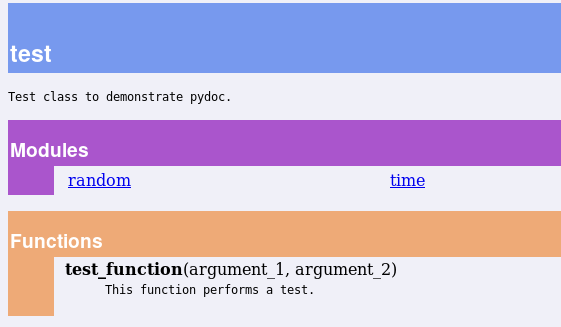
\includegraphics[width=0.8\textwidth]{08_Standard_Library/pydoc.png}

    \note{

        If you are using e.g. Firefox, you can just open the file from the terminal with \texttt{firefox test.html}.

    } 

\end{frame}


\section{The Python Standard Library}

\begin{frame}[plain]
    \sectionpage
\end{frame}

\begin{frame}[fragile]{The Python Standard Library}

    
    \includegraphics[width=0.8\textwidth]{08_Standard_Library/wc.png}


    \note{

        The packages that are included in every Python installation are called the Python Standard Library.

        \vspace{1em}

        You can find a list of them here:

        \url{https://docs.python.org/3/library/}

        \vspace{1em}

        To show all packages (modules) available in your local Python installation, open the Python shell and enter \texttt{help("modules")}
        
    }

\end{frame}

\begin{frame}[fragile]{What are packages?}

    \textbf{Packages} are collections of functions that are not automatically included in Python because they are too specialized.

    \vspace{1em}

    We distinguish between the packages included in the \texttt{Standard Library} ("inbuilt") and the ones that we first have to install ("external").

    \vspace{1em}

    Especially external packages can provide a lot of utility and efficiency, since they are often implemented in C, another programming language.

    \vspace{1em}

    In this lecture we will only talk about the packages in the \textbf{Standard Library}.

    \note{
        
        Installing external packages is in principle easy, especially if you already installed \texttt{conda}. 

        \vspace{1em}

        However, in practice many specialized external packages do not run properly on Windows.

        \vspace{1em}

        In lecture 13 we will give an introduction to an external package of your preference.

    }

\end{frame}


\begin{frame}[fragile]{Importing Packages}

    \textbf{There are three ways to access functions from packages:}

    \begin{itemize}

        \item Import the whole package: \texttt{import my\_package} 
              \newline $\Rightarrow$ Use \texttt{my\_package.my\_function()} to access any function

        \item Import specific function: \texttt{from my\_package import my\_function} 
              \newline $\Rightarrow$ Use \texttt{my\_function()} to access this function


        \item Import all functions: \texttt{from my\_package import *} 
              \newline $\Rightarrow$ Use \texttt{my\_function()} to access any function

    \end{itemize}

    \textbf{Import statements should always be at the top of your script.} 

    \note{

        \textbf{Never place import statements inside a loop or function definition.}

        \vspace{1em}

        \texttt{from X import *} is usually not the best idea because it means including a lot of functions that you probably do not need.

    }

\end{frame}


\begin{frame}[fragile]{Import Examples}

    \begin{pythoncode}

import turtle
turtle.forward(10)

from turtle import right
right(90)

from turtle import *
left(30)

    \end{pythoncode}

    Other packages from the Standard Library we already know are 

    \texttt{random}, \texttt{re}, \texttt{csv} and \texttt{json}

    \note{
        
        As said on the slide before, imports should always be performed at the top of your script.

        \vspace{1em}

        The only reason this is not done here is for demonstration purposes.

    }

\end{frame}

\section{copy}

\begin{frame}[plain]
    \sectionpage
\end{frame}

\begin{frame}[fragile]{\texttt{copy}}

    As you may have noticed, mutable data structures such as \texttt{lists} and \texttt{dictionaries} can behave unexpectedly:
    
    \begin{pythoncode}

my_list = [1, 2, 3]
banana = my_list

print(banana, my_list)
# Output: [1, 2, 3] [1, 2, 3]

banana[0] = 999

print(banana, my_list)
# Output: [999, 2, 3] [999, 2, 3]

    \end{pythoncode}

    \note{

        For immutable data structures, we never have the chance to experience this anomaly, 
        since they cannot be changed at all.

    }

\end{frame}


\begin{frame}[fragile]{\texttt{copy}}

    This is because \texttt{banana = my\_list} does not actually create a new list filled with the same values as \texttt{my\_list} to \texttt{banana},
    but instead they now both reference the same \textbf{list object}.


    \vspace{1em}

    In order to make an actual copy (a new list object filled with the same values), we have to use the package \texttt{copy}.


\end{frame}


    \note{

        You can find more information about \texttt{copy} here: 

        \url{https://docs.python.org/3/library/copy.html}

        \vspace{1em}
        
        This is closely related to the topic of Object-Oriented Programming, which will be covered in the next lecture.

    }


\begin{frame}[fragile]{\texttt{copy}}

    \begin{pythoncode}

from copy import copy

my_list = [1, 2, 3]
banana = copy(my_list)

print(banana, my_list)
# Output: [1, 2, 3] [1, 2, 3]

banana[0] = 999

print(banana, my_list)
# Output: [999, 2, 3] [1, 2, 3]

    \end{pythoncode}

    \note{

        The result is called a \textit{shallow copy}.

        \vspace{1em}

        Note that this only works with one-dimensional lists. In order to copy nested multi-dimensional lists, we need to the function \texttt{deepcopy}.

    }

\end{frame}


\begin{frame}[fragile]{\texttt{copy}}

    \begin{pythoncode}

from copy import copy

my_list = [[1, 2], [3, 4]]
banana = copy(my_list)

print(banana, my_list)
# Output: [[1, 2], [3, 4]] [[1, 2], [3, 4]]

banana[0][0] = 999

print(banana, my_list)
# Output: [[999, 2], [3, 4]] [[999, 2], [3, 4]]

    \end{pythoncode}

    \note{
    
        The result is called a \textit{shallow copy}.

        \vspace{1em}

        Note that this only works with one-dimensional lists. In order to copy nested multi-dimensional lists, we need the function \texttt{deepcopy}.

    }

\end{frame}


\begin{frame}[fragile]{\texttt{deepcopy}}

    \begin{pythoncode}

from copy import deepcopy

my_list = [[1, 2], [3, 4]]
banana = deepcopy(my_list)

print(banana, my_list)
# Output: [[1, 2], [3, 4]] [[1, 2], [3, 4]]

banana[0][0] = 999

print(banana, my_list)
# Output: [[999, 2], [3, 4]] [[1, 2], [3, 4]]

    \end{pythoncode}

    \note{
    
        The result is called a \textit{deep copy}. 

        \vspace{1em}

        This would also work on nested lists with more than two dimensions, as well as on lists of dictionaries etc.

    }

\end{frame}


\section{os and shutil}

\begin{frame}[plain]
    \sectionpage
\end{frame}

\begin{frame}[fragile]{\texttt{os}}

    \texttt{os.listdir()}, \texttt{os.mkdir()}, \texttt{os.rmdir()} and \texttt{os.remove()} 

    allow you to view, create and remove folders and files.

    \begin{pythoncode}

import os

print(os.listdir())
# Output: ['iai', 'bpp', 'a.txt', 'test.py']

os.mkdir("banana")
os.remove('a.txt')

print(os.listdir())
# Output: ['iai', 'bpp', 'test.py', 'banana']

    \end{pythoncode}

    \note{

        \textbf{Caution:} Especially with \texttt{os.remove()} and \texttt{os.rmdir()}, you can break a lot on your computer.

        \vspace{1em}

        \textbf{Files removed with os.rmdir() do not go into the recycle bin, but are deleted permanently.}
    
        \vspace{1em}

        You can find more information about \texttt{os} here: 

        \url{https://docs.python.org/3/library/os.html}

        \vspace{1em}

        The command-line equivalent of \texttt{os.listdir()} is \texttt{ls} in Linux and \texttt{dir} in Windows.

    }

\end{frame}

\begin{frame}[fragile]{Paths}

    We often use \textbf{paths} to tell Python where to look for files and folder locations. For each location, there are two ways to do this: 

    \vspace{1em}

    \begin{itemize}

        \item \textbf{Absolute Path}: The location is described by listing how to get there from the root directory, e.g. C: on Windows
        \item \textbf{Relative Path}: The location is described by listing how to get there from the current working directory

    \end{itemize}

    The current working directory is usually the folder in which you executed your Python code. You can access it with \texttt{os.getcwd()}.

    \note{

        You can find more information about \texttt{os} here: 

        \url{https://docs.python.org/3/library/os.html}

        \vspace{1em}

        Before sharing code you should always make sure that all your paths are relative, otherwise they may not be executable for others.

        \vspace{1em}
        
        Most functions related to files take as argument either a relative or an absolute path. 
        If no path is specified, the current working directory is automatically selected.

        \vspace{1em}

        The command-line equivalent of \texttt{os.getcwd()} in Linux is \texttt{pwd}. In Windows, depending on your version \texttt{cd} may produce the same result.

    }


\end{frame}

\begin{frame}[fragile]{Paths}

    The absolute path can be calculated from the relative path and the current working directory.

    \begin{pythoncode}

import os

relative_path = "my_folder/my_file.txt"

print(os.getcwd())
# Output: /home/nathan/teaching/

print(os.getcwd() + "/" + relative_path)
# Output: /home/nathan/teaching/my_folder/my_file.txt

    \end{pythoncode}

    \note{

        One example of where we have to use paths would be \texttt{open()}.

        \vspace{1em}
        
        Most functions related to files take as argument either a relative or an absolute path. 
        If no path is specified, the current working directory is automatically selected.

        \vspace{1em}

        The command-line equivalent of \texttt{os.getcwd()} in Linux is \texttt{pwd}. In Windows, depending on your version \texttt{cd} may produce the same result.

    }


\end{frame}

\begin{frame}[fragile]{\texttt{shutil}}

    \texttt{shutil.copy()} and \texttt{shutil.move()} allow you to move files.

    \begin{pythoncode}

import shutil
import os

print(os.listdir())
# Output: ['iai', 'bpp', 'a.txt', 'test.py']

os.mkdir("banana")
shutil.move("a.txt", "banana/a.txt")

print(os.listdir("banana"))
# Output: ['a.txt']

    \end{pythoncode}

    \note{

        You can find more information about \texttt{shutil} here: 

        \url{https://docs.python.org/3/library/shutil.html}

        \vspace{1em}
    
    }

\end{frame}


\section{math}

\begin{frame}[plain]
    \sectionpage
\end{frame}

\begin{frame}[fragile]{\texttt{math}}

    The \texttt{math} package is useful when implementing formulas

    \begin{itemize}

        \item It provides mathematical constants like \texttt{pi} and \texttt{e}
        \item It provides mathematical functions like \texttt{log} and \texttt{cos}
        \item It provides utilities like \texttt{ceil} and \texttt{floor}

    \end{itemize}

    \begin{pythoncode}

from math import log

print(log(5, 2))
# Output: 1.6094...
# Returns log2(5)

    \end{pythoncode}

    \note{

        You can find more information about \texttt{math} here: 

        \url{https://docs.python.org/3/library/math.html}

        \vspace{1em}

        With just one argument, \texttt{math.log(x)} returns the natural logarithm ln(x).

    }

\end{frame}


\begin{frame}[fragile]{\texttt{math}}

    \begin{pythoncode}

import math

print(math.pi)
# Output: 3.1415...

print(math.floor(2.6))
# Output: 2

print(math.ceil(2.6))
# Output: 3

    \end{pythoncode}

    \note{

        You can find more information about \texttt{math} here: 

        \url{https://docs.python.org/3/library/math.html}

        \vspace{1em}

        \texttt{math.floor()} returns the same value as \texttt{int}.

    }

\end{frame}


\section{time}

\begin{frame}[plain]
    \sectionpage
\end{frame}

\begin{frame}[fragile]{\texttt{time}}

    \texttt{time} provides many functions to calculate with all sorts of time formats.

    \begin{pythoncode}

import time

print(time.time())
# Output: 1558904793.3782952
# These are the seconds that have passed 
# since January 1st 1970 00:00:00

time.sleep(2)
# The script will now pause for 2 seconds


    \end{pythoncode}

    \note{

        You can find more information about \texttt{time} here: 

        \url{https://docs.python.org/3/library/time.html}

        \vspace{1em}

        January 1st 1970 00:00:00 is called the \textbf{epoch}.
    
    }

\end{frame}


\begin{frame}[fragile]{\texttt{time}}

    \texttt{time()} is useful when you want to time your code.

    \begin{pythoncode}

import time

def my_function():
    for n in range(100000):
        n += 2 * n

start_time = time.time()
my_function()

print("{:.4f} seconds".format(time.time() - start_time))
# Output: 0.5561 seconds

    \end{pythoncode}

    \note{

        You can find more information about \texttt{time} here: 

        \url{https://docs.python.org/3/library/time.html}
    
    }

\end{frame}


\begin{frame}[fragile]{\texttt{time}}

    \texttt{time} can also give you the time in a more human-readable form.

    \begin{pythoncode}

import time

now = time.localtime()
print(now)
# Output: time.struct_time(tm_year=2019, tm_mon=5, ...)

print(now.tm_year)
# Output: 2019

print(type(now.tm_year))
# Output: <class 'int'>

    \end{pythoncode}

    \note{


        The \texttt{something.attribute} notation is already a peek at next week's topic:

        \vspace{1em}

        \textbf{Object-Oriented Programming}
    
    }

\end{frame}


\section{sys}

\begin{frame}[plain]
    \sectionpage
\end{frame}

\begin{frame}[fragile]{\texttt{sys}}

    \texttt{argv} can be used to access command-line arguments passed to a script. This avoids the sometimes tedious use of \texttt{input()}.

    \vspace{1em}

    \texttt{python my\_script.py "hello!" 42}

    \begin{pythoncode}

import sys

print(sys.argv)
# Output: ['my_script.py', 'hello!', '42']
# The first argument is always the name of the script

print(len(sys.argv))
# Output: 3

    \end{pythoncode}

    \note{

        You can find more information about \texttt{sys} here: 

        \url{https://docs.python.org/3/library/sys.html}

        \vspace{1em}

        \texttt{sys} is much more powerful than that.

        \vspace{1em}

        \texttt{sys} can for example give you information about which operating system
        the script is run on and with which Python version.

    }

\end{frame}


\section{Organisational}

\begin{frame}[plain]
    \sectionpage
\end{frame}

\begin{frame}[fragile]{Schedule}

    \begin{enumerate}

        \setcounter{enumi}{1}
        \item Variables and Assignments
        \item Control Structures
        \item Data Structures
        \item Strings
        \item Input and Output
        \item Good Practices
        \item Standard Library
        \item Object-Oriented Programming
        \item Recap
        \item Pythonic Programming
        \item Using APIs
        \item \texttt{"\{\}".format(topic\_of\_your\_choice)}

    \end{enumerate}


\end{frame}


\begin{frame}[fragile]{Passing the Course}

    To pass this course, you need 10 homework points. Each sheet you passed gives you 1 homework point.

    \vspace{1em}

    To pass a sheet, you need at least 60 percent of the points.

    \vspace{1em}

    There are 5 regular sheets left.

    \vspace{1em}

    There will be the option to hand in a project for 2 - 3 homework points at the end of the semester.
    
    \vspace{1em}

    We will discuss the projects in the Recap lecture on June 12th.

    \note{

        If you have any problems, you can always send us a message.

        \vspace{1em}

        Or better yet, request a feedback session via the StudIP groups!

        \vspace{1em}

        You can reach us here:

        \begin{itemize}

            \item mpoemsl@uos.de
            \item kgross@uos.de
            \item sselbach@uos.de
        
        \end{itemize}

    }


\end{frame}


\begin{frame}[fragile]{Passing the Course}

    
    \vspace{1em}

    \textbf{There will be no practice session this week due to the holiday!}


    \note{

        If you have any problems, you can always send us a message.

        \vspace{1em}

        Or better yet, request a feedback session via the StudIP groups!

        \vspace{1em}

        You can reach us here:

        \begin{itemize}

            \item mpoemsl@uos.de
            \item kgross@uos.de
            \item sselbach@uos.de
        
        \end{itemize}

    }


\end{frame}


\end{document}
